%Update 10/10/2022
\documentclass{article}     %type of document
\usepackage[utf8]{inputenc} %for text encoding
\usepackage{../lambdatex}

\title{Teoremi di Analisi}
\author{Davide Borra - 5LA}
\date{A.S. 2021-2022}

\everymath{\displaystyle}

\begin{document}
\lhead{Teoremi di Analisi}
\chead{}
\rhead{Davide Borra - 5LA}
\begin{titlepage}
    \maketitle
    \tableofcontents
    \hspace{\fill} v. 3.1   %incrementare primo numero per contenuti e secondo numero per patch
\end{titlepage}
\section{Primi teoremi sui limiti}
\textbf{N.B.:} I seguenti teoremi valgono per ogni tipologia di limite, sia finito che infinito, e in ogni intorno, sia di un numero reale (anche destro e sinistro) sia di infinito.
    \subsection{Teorema di unicità del limite}
        \begin{shadedTheorem}[Unicità del limite]
            Se una funzione $f(x)$ ha limite finito per $x$ che tende a $x_0$, allora tale limite è unico.
        \end{shadedTheorem}
        \begin{tabular}{m{0.48\textwidth}m{0.48\textwidth}}
            \textit{Ipotesi} & \textit{Tesi}  \\
            $\displaystyle\lim_{x\rightarrow x_0}f(x) = l$ & $l$ è unico
        \end{tabular}
        
        \begin{proof}
        Si procede per assurdo. Si supponga che 
        \[\lim_{x\rightarrow x_0}f(x) = l~~~~\land~~~~ \lim_{x\rightarrow x_0}f(x) = l'\]
        con $l\neq l'$ e $l<l'$.
        Siccome $\varepsilon$ è una quantità arbitraria è possibile porre \[0<\varepsilon<\frac{l-l'}{2}\]
        Si applicano ora le definizioni di limite:
        \[\forall \varepsilon > 0 ~~\exists I(x_0) : |f(x)-l|<\varepsilon~~\forall x \in I(x_0), x\neq x_0\]
        \[\forall \varepsilon > 0 ~~\exists I(x_0) : |f(x)-l'|<\varepsilon~~\forall x \in I(x_0), x\neq x_0\]
        Siccome l'intersezione di due intorni di $x_0$ è ancora un intorno di $x_0$, devono valere entrambe le definizioni:
        \[\left\{\begin{array}{l}
            l-\varepsilon < f(x) < l+\varepsilon\\
            l'-\varepsilon < f(x) < l'+\varepsilon 
        \end{array}\right.\]
        \\Ricordando che $l-\varepsilon<l'-\varepsilon < l+\varepsilon < l'+\varepsilon$ si ottiene:
        \[l'-\varepsilon < f(x) < l+\varepsilon\]
        \[l'-\varepsilon < l+\varepsilon\]
        \[-2\varepsilon<l-l'\]
        \[2\varepsilon > l'-l\]
        \[\varepsilon > \frac{l'-l}{2}\]
        Assurdo: contrasta con quanto posto all'inizio. L'ipotesi per assurdo è falsa, quindi la tesi è dimostrata.\\
        \end{proof}
        
    \subsection{Teorema di permanenza del segno}
        \begin{shadedTheorem}[Permanenza del segno]
            Se il limite di un funzione per $x$ che tende a $x_0$ è un numero $l$ diverso da 0, allora esiste un intorno $I(x_0)$ escluso al più $x_0$ in cui $f(x)$ e $l$ sono entrambi positivi o entrambi negativi.
        \end{shadedTheorem}
        \begin{tabular}{m{0.48\textwidth}m{0.48\textwidth}}
            \textit{Ipotesi} & \textit{Tesi}  \\
            $\displaystyle\lim_{x\rightarrow x_0}f(x) = l ~~ \land ~~ l\neq 0$ & $\exists I(x_0) : f(x) \text{ e } l \text{ sono concordi}~~\forall x \in I(x_0), x\neq x_0$
        \end{tabular}
        
        \begin{proof}
        Espando l'ipotesi:
        \[\forall \varepsilon > 0 ~~\exists I(x_0) : |f(x)-l|<\varepsilon~~\forall x \in I(x_0), x\neq x_0\]
        Siccome $\varepsilon$ è un numero positivo arbitrario pongo 
        \[\varepsilon = |l|\]
        \[|f(x)-l|<\varepsilon\]
        \[-\varepsilon <f(x)-l<\varepsilon\]
        \[l-\varepsilon<f(x)<l+\varepsilon\]
        \begin{itemize}
            \item se $l>0 \rightarrow \varepsilon =l$
            \[l-l<f(x)<l+l\]
            \[0<f(x)<2l\]
            da cui la tesi\[f(x)>0\]
            \item se $l<0 \rightarrow \varepsilon =-l$
            \[l+l<f(x)<l-l\]
            \[2l<f(x)<0\]
            da cui la tesi\[f(x)<0\]
        \end{itemize}
        \end{proof}
        
        \begin{shadedTheorem}[Inverso della permanenza del segno]
            Se una funzione $f(x)$ ammette limite finito $l$ per $x$ che tende a $x_0$ e in un intorno $I(x_0)$ escluso al più $x_0$ è 
            \begin{itemize}
                \item positiva o nulla, allora $l\geq 0\lor l=+\infty$;
                \item negativa o nulla, allora $l\leq 0\lor l=-\infty$.
            \end{itemize}
        \end{shadedTheorem}
        
    \subsection{Teorema del confronto (o dei due carabinieri)}
        \begin{shadedTheorem}[Confronto]
            Siano $g(x)$, $f(x)$ e $h(x)$ tre funzioni definite in uno stesso intorno $I(x_0)$, escluso al più $x_0$. Se per ogni $x\in I(x_0)$ è verificato che \[g(x)\leq f(x) \leq h(x)\]
            e \[\lim_{x\rightarrow x_0} g(x)=l ~~ \land ~~ \lim_{x\rightarrow x_0} h(x)=l\]
            allora è verificato che
            \[\lim_{x\rightarrow x_0} f(x)=l\].
        \end{shadedTheorem}
        \begin{tabular}{m{0.45\textwidth}m{0.45\textwidth}}
            \textit{Ipotesi} & \textit{Tesi}  \\
            \begin{enumerate}
                \item $g(x)$, $f(x)$ e $h(x)$ tre funzioni definite nello stesso intorno $I(x_0)$
                \item $\forall x \in I(x_0) ~~ g(x)\leq f(x) \leq h(x)$
                \item $\displaystyle\lim_{x\rightarrow x_0} g(x)=l ~~ \land ~~ \lim_{x\rightarrow x_0} h(x)=l$
            \end{enumerate} & \[\lim_{x\rightarrow x_0} f(x)=l\]\\
        \end{tabular}
        
        \begin{proof}
            Espando l'ipotesi 3:
            \[\forall \varepsilon > 0 ~~\exists I(x_0) : |g(x)-l|<\varepsilon~~\forall x \in I(x_0), x\neq x_0\]
            \[\forall \varepsilon > 0 ~~\exists I(x_0) : |h(x)-l|<\varepsilon~~\forall x \in I(x_0), x\neq x_0\]
            Di conseguenza 
            \[l-\varepsilon < g(x) <l+\varepsilon\]
            \[l-\varepsilon < h(x) <l+\varepsilon\]
            da cui, per ipotesi 1, 
            \[l-\varepsilon < g(x)\leq h(x) <l+\varepsilon\]
            \[l-\varepsilon < g(x) \leq f(x) \leq h(x) <l+\varepsilon\]
            \[l-\varepsilon < f(x) <l+\varepsilon\]
            La precedente scrittura è equivalente a 
            \[|f(x)-l|<\varepsilon\]
            da cui la tesi.\\
        \end{proof}
    
\section{Continuità e funzioni inverse}
    \subsection{Continuità della funzione inversa}
        \begin{shadedTheorem}[Continuità della funzione inversa]
            Se $y=f(x)$ è una funzione biiettiva e continua in un intervallo $D$, allora la funzione inversa $f^{-1}$ è continua nel codominio di $f$.
        \end{shadedTheorem}
        \begin{tabular}{m{0.45\textwidth}m{0.45\textwidth}}
            \textit{Ipotesi} & \textit{Tesi}  \\
            $f:D\to C$ biiettiva e continua in D & $f^{-1}:C\to D$ continua in C 
        \end{tabular}
        
    \subsection{Condizione di invertibilità per funzioni continue}
        \begin{shadedTheorem}[Invertibilità di funzioni continue]
            Sia $I$ un intervallo (limitato o illimitato) e $f:I\rightarrow \R$ una funzione continua in $I$. Allora essa è invertibile se e solo se è strettamente monotona.
        \end{shadedTheorem}
        \begin{tabular}{m{0.45\textwidth}m{0.45\textwidth}}
            \textit{Ipotesi} & \textit{Tesi}  \\
            $f:I\to \R$ continua e strettamente monotona in $I$ & $f$ è invertibile 
        \end{tabular}
    
\section{Teoremi sulle funzioni continue}
    \subsection{Teorema di Weistrass}
        \begin{shadedTheorem}[Weistrass]
            Se $f$ è una funzione continua in un intervallo limitato e chiuso $[a;b]$, allora essa assume in tale intervallo il massimo assoluto e il minimo assoluto.
        \end{shadedTheorem}
        \begin{tabular}{m{0.45\textwidth}m{0.45\textwidth}}
            \textit{Ipotesi} & \textit{Tesi}  \\
            $f:[a;b]\to \R$ continua in $[a;b]$ & $\exists c,d \in [a,b] : f(c) = min\{f\} \land f(d) = max\{f\}$
        \end{tabular}
    
    \subsection{Teorema dell'esistenza degli zeri (o di Bolzano)}
        \begin{shadedTheorem}[Bolzano]
            Se $f$ è continua in un intervallo limitato e chiuso $[a;b]$ e negli estremi di tale intervallo assume valori di segno opposto, allora esiste almeno un punto $c$ interno all'intervallo in cui $f(c)=0$.
        \end{shadedTheorem}
        \begin{tabular}{m{0.45\textwidth}m{0.45\textwidth}}
            \textit{Ipotesi} & \textit{Tesi}  \\
            \begin{enumerate}
                \item $f: [a;b] \to \R$ continua in $[a;b]$
                \item $f(a) \cdot f(b)<0$
            \end{enumerate} & $\exists c \in [a;b]:f(c)=0$ 
        \end{tabular}
    
    \subsection{Teorema dei valori intermedi (o di Darboux)}
        \begin{shadedTheorem}[Darbaux]
            Se $f$ è una funzione continua in un intervallo limitato e chiuso $[a;b]$, allora essa assume almeno una volta tutti i valori compresi tra il massimo e il minimo.
        \end{shadedTheorem}
        \begin{tabular}{m{0.45\textwidth}m{0.45\textwidth}}
            \textit{Ipotesi} & \textit{Tesi}  \\
            \begin{enumerate}
                \item $f: [a;b]\to \R$ continua in $[a;b]$
                \item $m=min\{[a;b]\}$ ~~~ $M=max\{[a;b]\}$
            \end{enumerate} & $\exists x \in [a,b] : f(x)=k \forall k \in [m;M]$
        \end{tabular}
    
\section{Legame tra continuità e derivabilità}
    \subsection{Continuità delle funzioni derivabili}
        \begin{shadedTheorem}[Continuità delle funzioni derivabili]
            Se una funzione $f(x)$ è derivabile nel punto $x_0$ allora in quel punto la funzione è anche continua.
        \end{shadedTheorem}
        \begin{tabular}{m{0.45\textwidth}m{0.45\textwidth}}
            \textit{Ipotesi} & \textit{Tesi}  \\
            $\exists f'(x_0)$ & $f(x)$ è continua in $x_0$
        \end{tabular}
        \begin{proof}
        \[f(x_0+h)=f(x_0+h)\]
        \[f(x_0+h)=f(x_0+h)-f(x_0)+f(x_0)\]
        \[f(x_0+h)=\frac{f(x_0+h)-f(x_0)}{h}\cdot h+f(x_0), ~~~~\text{con } h\neq 0\]
        Calcolo i limiti dei membri per $h \to 0$
        \[\lim_{h\to 0}f(x_0+h)=\lim_{h\to0}\left[\frac{f(x_0+h)-f(x_0)}{h}\cdot h+f(x_0)\right]\]
        Siccome a secondo membro il limite è la somma di limiti finiti, posso separarli
        \[\lim_{h\to 0}f(x_0+h)=\lim_{h\to0}\frac{f(x_0+h)-f(x_0)}{h}\cdot h+\lim_{h\to0}f(x_0)\]
        Siccome non si presentano forme di indecisione posso separare:
        \[\lim_{h\to 0}f(x_0+h)=f'(x_0)\cdot \lim_{h\to0} h+\lim_{h\to0}f(x_0)\]
        \[\lim_{h\to 0}f(x_0+h)=f(x_0)\]
        pongo $x_0+h = x$, per cui $h=x-x_0$. Se $h\to 0$, $x\to x_0$
        \[\lim_{x\to x_0}f(x) = f(x_0)\]
        \end{proof}
    \subsection{Criterio di derivabilità}
        \begin{shadedTheorem}[Criterio di derivabilità]
            Sia $f(x)$ una funzione continua in $[a;b]$ e derivabile in $]a;b[$ tranne al più $x_0$ (con $x_0\in ]a;b[$). Allora 
            \[f'_-(x_0)=\lim_{x\to x_0^-}f'(x) ~~~\land~~~ f'_+(x_0)=\lim_{x\to x_0^+}f'(x)\]
            In particolare se $f'_+(x_0) = f'_-(x_0)$ e sono finite, allora la funzione è derivabile in $x_0$ e $f'(x_0)=f'_+(x_0) = f'_-(x_0)$.
        \end{shadedTheorem}
        \begin{tabular}{m{0.45\textwidth}m{0.45\textwidth}}
            \textit{Ipotesi} & \textit{Tesi}  \\
            \begin{enumerate}
                \item $f(x)$ continua in $[a;b]$
                \item $f(x)$ derivabile in $]a;b[-\{x_0\}$ (con $x_0\in]a;b[$)
            \end{enumerate} & \begin{enumerate}
                \item $f'_-(x_0)=\lim_{x\to x_0^-}f'(x)$
                \item $f'_+(x_0)=\lim_{x\to x_0^+}f'(x)$
            \end{enumerate}\\
            \textit{Ipotesi 2} & \textit{Tesi 2}  \\
            $f'_+(x) = f'_-(x)$ e finite & \begin{enumerate}
                \item $f(x)$ derivabile in $x_0$
                \item $f'(x_0)=f'_+(x_0) = f'_-(x_0)$
            \end{enumerate}
        \end{tabular}

\section{Teoremi del calcolo differenziale}
    \subsection{Teorema di Fermat}
        \begin{shadedTheorem}[Fermat]
            Data una funzione $y=f(x)$ definita in un intervallo $[a;b]$ e derivabile in $]a;b[$, se $f(x)$ ha un massimo o un minimo relativo nel nel punto $x_0$ interno ad $[a;b]$, allora la derivata della funzione in quel punto si annulla.
        \end{shadedTheorem}
        \begin{tabular}{m{0.60\textwidth}m{0.30\textwidth}}
            \textit{Ipotesi} & \textit{Tesi}  \\
            \begin{enumerate}
                \item $f:[a;b]\to\R$
                \item $f(x)$ derivabile in $]a;b[$
                \item $x_0$ punto di massimo o minimo relativo ($x_0\in [a;b]$)
            \end{enumerate} & $f'(x_0)=0$
        \end{tabular}\\
        \textbf{N.B.:} La dimostrazione è svolta considerando $x_0$ punto di massimo, ma lo svolgimento è analogo nel caso di un punto di minimo.
        \InsertBoxR{2}{\begin{minipage}{0.30\linewidth}\centering
            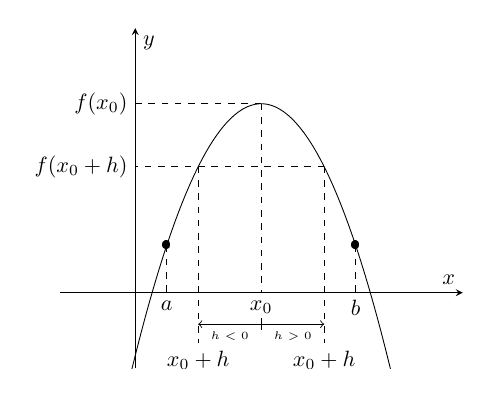
\begin{tikzpicture}[scale = 0.8]
                \begin{axis}[
                    x=1.0cm,y=1.0cm,
                    axis lines=middle,
                    xlabel = $x$,
                    ylabel =$y$,
                    xmin=-1.7,
                    xmax=5.2,
                    ymin=-1.2,
                    ymax=4.2,
                    xtick={-10.0,0.0,...,10.0},
                    ytick={-10.0,0.0,...,10.0},]
                    \draw [samples=100, domain=-1.2:5.2] plot(\x,{-((\x)-2)^2+3});
                    \draw[dashed] (2,3) -- (0,3) node[left]{$f(x_0)$};
                    \draw[dashed] (2,3) -- (2,0) node[below]{$x_0$};
                    \draw[dashed] (3, 2) -- (0,2) node[left]{$f(x_0+h)$}; 
                    \draw[color=white, ultra thick] (-1.2,0)--(-1.7,0);
                    \draw[dashed] (1, 2) -- (1,-0.8) node[below]{$x_0+h$}; 
                    \draw[dashed] (3, 2) -- (3,-0.8) node[below]{$x_0+h$}; 
                    \draw[->] (2,-0.5) --node[below]{\tiny$ h<0$} (1,-0.5);
                    \draw[->] (2,-0.5) --node[below]{\tiny$ h>0$} (3,-0.5);
                    \draw (2,-0.4)--(2,-0.6);
                    \draw[dashed] (0.5, 0.75) -- (0.5,0) node[below]{$a$}; 
                    \draw[dashed] (3.5, 0.75) -- (3.5,0) node[below]{$b$};
                    \node at (0.5, 0.75){\textbullet}; 
                    \node at (3.5, 0.75){\textbullet};
                 \end{axis}
            \end{tikzpicture}
        \end{minipage}}
        \begin{proof}
        Per definizione di punto di massimo relativo
        \[f(x) \leq f(x_0) ~~~~\forall x \in I(x_0)\]
        \[f(x_0+h)\leq f(x_0)\]
        \[f(x_0+h)-f(x_0)\leq 0~~~~ \forall h \in \R\]
        Calcolo i rapporti incrementali da sinistra e da destra:
        \[\mathbf{h>0}~~~~ \frac{f(x_0+h)-f(x_0)}{h}\leq 0\]
        \[\mathbf{h<0}~~~~ \frac{f(x_0+h)-f(x_0)}{h}\geq 0\]
        Per l'inverso del teorema della permanenza del segno:
        \[f'_+(x_0)=\lim_{h\to 0^+}\frac{f(x_0+h)-f(x_0)}{h}\leq 0\]
        \[f'_-(x_0)=\lim_{h\to 0^-}\frac{f(x_0+h)-f(x_0)}{h}\geq 0\]
        Siccome $f(x)$ è derivabile per ipotesi 2, per il criterio di derivabilità
        \[f'_+(x_0)=f'_-(x_0)\]
        Di conseguenza è necessario che \[f'_+(x_0)=f'_-(x_0)=f'(x_0)=0\].
        \end{proof}
        
    \subsection{Teorema di Rolle}
        \begin{shadedTheorem}[Rolle]
        Data una funzione $y=f(x)$ definita in un intervallo limitato e chiuso $[a;b]$ tale che \begin{enumerate}
            \item $f(x)$ è continua in $[a;b]$
            \item $f(x)$ è derivabile in $]a;b[$
            \item $f(a)=f(b)$
        \end{enumerate}
        allora esiste almeno un punto $c$ interno all'intervallo per il quale risulta $f'(c)=0$
        \end{shadedTheorem}
        \begin{tabular}{m{0.45\textwidth}m{0.45\textwidth}}
            \textit{Ipotesi} & \textit{Tesi}  \\
            \begin{enumerate}
            \item $f:[a;b] \to \R$
            \item $f(x)$ continua in $[a;b]$
            \item $f(x)$ derivabile in $]a;b[$
            \item $f(a)=f(b)$
        \end{enumerate} & $f'(c)=0$
        \end{tabular}
        
        \begin{proof}
        Dato che per ipotesi $f(x)$ è continua in un intervallo chiuso e limitato $[a;b]$ allora per il teorema di Weistrass $f(x)$ ammette massimo e minimo \textbf{assoluti} in tale intervallo, cioè \[\exists c,d \in [a;b] : m=f(c)\leq f(x)\leq f(d) = M\]
        \begin{figure}
            \centering
            %FIGURA
        \end{figure}
        Possiamo distinguere due casi:
        \begin{enumerate}
            \item $\mathbf{m=M}\to m=f(c)= f(x)= f(d) = M$\\
            Se $m$ e $M$ coincidono vuol dire che $f(x)$ assume sempre lo stesso valore. Dato che $f(x)$ deve essere compresa tra $m$ e $M$\[m\leq f(x) \leq M\]
            ma siccome $m=M$ allora $f(x)=m=M ~~\forall x \in [a;b]$, per cui $f(x)$ è costante. Siccome la derivata di una funzione costante è nulla \[f'(x)=0~~\forall x \in [a;b]\].
            \item $\mathbf{m<M}$, quindi $f(x)$ non è costante ($f(c)\neq f(d)$) e dato che sappiamo che $f(a)=f(b)$ allora \textbf{almeno} uno dei punti $c$ e $d$ deve essere interno all'intervallo $[a;b]$.\\ Supponiamo che $c\in ]a;b[$, quindi che $c$ non sia un estremo. In questo caso è possibile determinare un numero $h$ tale che $c-h$ e $c+h$ appartengano entrambi all'intervallo $[a;b]$. Siccome $c$ è un punto di minimo vale la relazione 
            \[f(x) \geq f(c) ~~~~ \forall x \in I(c)\]
            \[f(c+x)\geq f(c)\]
            \[f(c+h)-f(c)\geq 0 ~~~~\forall h \in \R\]
            Calcolo i rapporti incrementali da sinistra e da destra:
            \[\mathbf{h>0}~~~~ \frac{f(c+h)-f(c)}{h}\geq 0\]
            \[\mathbf{h<0}~~~~ \frac{f(c+h)-f(c)}{h}\leq 0\]
            Per l'inverso del teorema della permanenza del segno:
            \[f'_+(c)=\lim_{h\to 0^+}\frac{f(c+h)-f(c)}{h}\geq 0\]
            \[f'_-(c)=\lim_{h\to 0^-}\frac{f(c+h)-f(c)}{h}\leq 0\]
            Siccome $f(x)$ è derivabile per ipotesi 3, per il criterio di derivabilità
            \[f'_+(c)=f'_-(c)\]
            Di conseguenza è necessario che \[f'_+(c)=f'_-(c)=f'(c)=0\]
            La dimostrazione è analoga nel caso in cui $d$ e non $c$ appartenga all'intervallo $]a;b[$, e quindi si tratti di un punto di massimo e non di minimo.
        \end{enumerate}
        \end{proof}
    \subsection{Teorema di Lagrange}
        \begin{shadedTheorem}[Lagrange]
        Data una funzione $y=f(x)$ definita in un intervallo limitato e chiuso $[a;b]$ tale che \begin{enumerate}
            \item $f(x)$ è continua in $[a;b]$
            \item $f(x)$ è derivabile in $]a;b[$
        \end{enumerate}
        allora esiste almeno un punto $c$ interno all'intervallo per il quale vale la relazione \[\frac{f(b)-f(a)}{b-a}=f'(c)\]
        \end{shadedTheorem}
        \begin{tabular}{m{0.45\textwidth}m{0.45\textwidth}}
            \textit{Ipotesi} & \textit{Tesi}  \\
            \begin{enumerate}
            \item $f:[a;b] \to \R$
            \item $f(x)$ continua in $[a;b]$
            \item $f(x)$ derivabile in $]a;b[$
        \end{enumerate} & $\exists c \in~~]a;b[ ~~:~~ \dfrac{f(b)-f(a)}{b-a}=f'(c)$
        \end{tabular}
        \subsubsection*{Conseguenze del teorema di Lagrange}
        \subsubsection{Funzioni con derivata nulla}
            \begin{shadedTheorem}[Derivata nulla]
                Se $f(x)$ è una funzione continua in un intervallo $[a;b]$, derivabile in $]a;b[$ e la sua derivata è nulla per ogni punto interno all'intervallo, allora $f(x)$ è costante in tutto $[a;b]$
            \end{shadedTheorem}
            \begin{tabular}{m{0.45\textwidth}m{0.45\textwidth}}
                \textit{Ipotesi} & \textit{Tesi}  \\ 
                \begin{enumerate}
                \item $f:[a;b] \to \R$
                \item $f(x)$ continua in $[a;b]$
                \item $f(x)$ derivabile in $]a;b[$
                \item $f'(x)=0~~\forall x \in [a;b]$
        \end{enumerate} & $f(x)=k ~~ \forall x \in [a;b]$
           \end{tabular}
           
        \subsubsection{Funzioni con derivate uguali}
            \begin{shadedTheorem}[Differenza costante]
                Se $f(x)$ e $g(x)$ sono due funzioni continue nell'intervallo $[a;b]$, derivabili in $]a;b[$ e tali che $f'(x)=g'(x)~~\forall x \in ]a;b[$, allora esse differiscono per una costante.
            \end{shadedTheorem}
            \begin{tabular}{m{0.45\textwidth}m{0.45\textwidth}}
            \textit{Ipotesi} & \textit{Tesi}\\
            \begin{enumerate}
                \item $f:[a;b] \to \R$, $g: [a;b] \to \R$
                \item $f(x)$ continua in $[a;b]$
                \item $f(x)$ derivabile in $]a;b[$
                \item $g(x)$ continua in $[a;b]$
                \item $g(x)$ derivabile in $]a;b[$
                \item $f'(x)=g'(x) ~~ \forall x \in [a;b]$
        \end{enumerate} & $f(x)-g(x) = k ~~ \forall x \in [a;b]$
           \end{tabular}
        \subsubsection{Monotonia di funzioni derivabili}
            \begin{shadedTheorem}[Monotonia di funzioni derivabili]
                Data una funzione $y=f(x)$, continua e derivabile in un intervallo $[a;b]$ e derivabile nell'intervallo $]a;b[$: \begin{enumerate}
                    \item se $f'(x)>0 ~~\forall x \in ]a;b[$, allora $f(x)$ è crescente in $]a;b[$
                    \item se $f'(x)<0 ~~\forall x \in ]a;b[$, allora $f(x)$ è decrescente in $]a;b[$
                \end{enumerate} 
            \end{shadedTheorem}
            \begin{shadedTheorem}[Inverso della monotonia di funzioni derivabili]
                Data una funzione $y=f(x)$, continua e derivabile in un intervallo $[a;b]$ e derivabile nell'intervallo $]a;b[$: \begin{enumerate}
                    \item se $f(x)$ è crescente in $]a;b[$, allora $f'(x)\geq0 ~~\forall x \in ]a;b[$
                    \item se $f(x)$ è decrescente in $]a;b[$, allora $f'(x)\leq0 ~~\forall x \in ]a;b[$
                \end{enumerate} 
            \end{shadedTheorem}

        \subsection{Teorema di Cauchy}
        \begin{shadedTheorem}[Cauchy]
        Siano $y=f(x)$ e $y=g(x)$ due funzioni tali che 
        \begin{enumerate}
            \item $f(x)$ e $g(x)$ sono continue in $[a;b]$
            \item $f(x)$ e $g(x)$ sono è derivabili in $]a;b[$
            \item $g'(x)\neq 0 ~~ \forall x \in ]a;b[$ 
        \end{enumerate}
        allora esiste almeno un punto $c$ interno all'intervallo per il quale vale la relazione \[\frac{f(b)-f(a)}{g(b)-g(a)}=\frac{f'(c)}{g'(c)}\]
        \end{shadedTheorem}
        \begin{tabular}{m{0.45\textwidth}m{0.45\textwidth}}
            \textit{Ipotesi} & \textit{Tesi}  \\
            \begin{enumerate}
            \item $f:[a;b] \to \R$, $g: [a;b] \to \R$
            \item $f(x)$ continua in $[a;b]$
            \item $f(x)$ derivabile in $]a;b[$
            \item $g(x)$ continua in $[a;b]$
            \item $g(x)$ derivabile in $]a;b[$
            \item $g'(x)\neq 0 ~~ \forall x \in ]a;b[$
        \end{enumerate} & $\exists c \in~~]a;b[ ~~:~~ \dfrac{f(b)-f(a)}{g(b)-g(a)}=\dfrac{f'(c)}{g'(c)}$
        \end{tabular}

    \subsection{Teorema di De l'Hôpital}
    \textbf{N.B.:} Applicabile per la risoluzione delle forme di indecisione $\left[\frac{0}{0}\right]$ o $\left[\frac{\infty}{\infty}\right]$
        \begin{shadedTheorem}[De l'Hôpital]
            Date due funzioni $f(x)$ e $g(x)$ definite nell'intorno $I$ di un punto $x_0\in \overline{\R}$, se
            \begin{enumerate}
                \item $f(x)$ e $g(x)$ sono continue in $x_0$ e $f(x_0)=g(x_0)=0$ (o $\infty$)
                \item $f(x)$ e $g(x)$ sono derivabili in $I(x_0)-\{x_0\}$ 
                \item $g'(x)\neq 0$ in $I(x_0)-\{x_0\}$
                \item esiste $\lim_{x\to x_0}\frac{f'(x)}{g'(x)}$
            \end{enumerate}
            Allora esiste anche $\lim_{x\to x_0}    \frac{f(x)}{g(x)}$ e risulta:
            \[\lim_{x\to x_0}\frac{f(x)}{g(x)}\underset{\mathrm{H}}{=}\lim_{x\to x_0}\frac{f'(x)}{g'(x)}\]
        \end{shadedTheorem}
        \begin{tabular}{m{0.55\textwidth}m{0.35\textwidth}}
            \textit{Ipotesi} & \textit{Tesi}  \\
            \begin{enumerate}
                \item $f: I(x_0)\to \R$
                \item $g: I(x_0)\to \R$
                \item $f(x)$ e $g(x)$ continue in $x_0$ e $f(x_0)=g(x_0)=0$ (o $\infty$)
                \item $f(x)$ e $g(x)$ derivabili in $I(x_0)-\{x_0\}$ 
                \item $g'(x)\neq 0 ~~\forall~ x \in I(x_0)-\{x_0\}$
                \item $\exists \lim_{x\to x_0}\frac{f'(x)}{g'(x)}$
            \end{enumerate} & \[\lim_{x\to x_0}\frac{f(x)}{g(x)}\underset{\mathrm{H}}{=}\lim_{x\to x_0}\frac{f'(x)}{g'(x)}\]
        \end{tabular}
    
\section{Teoremi sugli integrali}
    \subsection{Teorema fondamentale del calcolo integrale}
        \begin{shadedTheorem}[Torricelli-Barrow]
            Se una funzione $f(x)$ è continua in $[a;b]$, allora esiste la derivata della sua funzione integrale
            \[F(x)=\int_a^x f(t)dt\]
            per ogni punto $x$ dell'intervallo $[a;b]$ ed è uguale a $f(x)$, cioè:
            \[F'(x)=f(x)\]
            ovvero $F(x)$ è una primitiva di $f(x)$.
        \end{shadedTheorem}
        \begin{tabular}{m{0.45\textwidth}m{0.45\textwidth}}
            \textit{Ipotesi} & \textit{Tesi}  \\
            \begin{enumerate}
                \item $f(x)$ continua in $[a;b]$
                \item $F(x)=\int_a^x f(t)dt$
            \end{enumerate} & 
            \begin{enumerate}
                \item $\exists~~ F'(x)$
                \item $F'(x)=f(x)$
            \end{enumerate}
        \end{tabular}
\end{document}